\documentclass[letterpaper, 12pt]{article}

\usepackage{geometry}
 \geometry{
 letterpaper,
 total={170mm,257mm},
 left=20mm,
 top=20mm,
 bottom=20mm
 }
\usepackage{graphicx} % Required for inserting images
\usepackage{authblk}
\usepackage{amssymb}
\usepackage{lipsum}
\usepackage{float}
\usepackage{times}
\usepackage{amsmath}
\usepackage[format=plain,
            labelfont={bf,it},
            textfont=it]{caption}
\captionsetup{justification=raggedright,singlelinecheck=false}
\usepackage{ragged2e}
\usepackage{longtable}
\usepackage{comment}
\usepackage{setspace}
\usepackage{fancyhdr}
\usepackage{titlesec}
\usepackage[hyperindex,breaklinks]{hyperref}
\hypersetup{
    colorlinks=true,
    linkcolor=blue,
    filecolor=magenta,      
    urlcolor=blue
    }
% \usepackage{background} % add COSIG logo to page
\usepackage[T1]{fontenc}
\usepackage{helvet}
\renewcommand{\familydefault}{\sfdefault}
\pagenumbering{gobble}
\usepackage[skip=10pt plus1pt, indent=40pt]{parskip}

\titlespacing*{\section}
{0pt}{1.5ex plus 1ex minus .2ex}{1.3ex plus .2ex}

\renewcommand\Authfont{\fontsize{12}{14.4}\selectfont}
\renewcommand\Affilfont{\fontsize{9}{10.8}\itshape}
 
\begin{document}
\flushleft

\includegraphics[width=0.5\textwidth]{img/home/241017_final_logo_mockup.png}

\section*{Granularity testing using GRIM and GRIMMER}
\addcontentsline{toc}{section}{Granularity testing using GRIM and GRIMMER}
\textit{Last updated: 03 June 2025}

Many quantitative research articles report the total number of observations (sample size), means, percentages, and/or standard deviations. Under certain conditions related to the granularity of the raw data, only some means, percentages, and standard deviations are possible for a given sample size. Under certain conditions, it is therefore possible to check whether reported means, percentages, or standard deviations are mathematically possible given reported sample sizes. 

These granularity-based methods for assessing consistency are referred to as GRIM (Granularity Related Inconsistency of Means: \href{https://jamesheathers.medium.com/the-grim-test-a-method-for-evaluating-published-research-9a4e5f05e870}{Heathers (2016a)}, \href{https://jamesheathers.medium.com/the-grim-test-further-points-follow-ups-and-future-directions-afd55ff67bb0#.vmgjvdvkf}{Heathers (2016b)}, \href{https://doi.org/10.1177/1948550616673876}{Brown \& Heathers (2017)}) and GRIMMER (an extension for standard deviations, see \href{https://aurelienallard.netlify.app/post/anaytic-grimmer-possibility-standard-deviations/}{Allard (2018)}; \href{https://peerj.com/preprints/2400/}{Anaya (2016)}; \href{https://jamesheathers.curve.space}{Heathers, (2025a)}). Checking for such inconsistencies between reported sample size and summary statistics can be an efficient and useful way of checking the trustworthiness of research \href{https://doi.org/10.1177/1948550616673876}{Brown, N., \& Heathers, J. (2017). 

GRIM and GRIMMER, which this guide collectively refers to as GRIM/MER, are useful because they do not require access to the raw data, only to numbers that are commonly reported in articles. This can be useful in the direct sense that GRIM/MER can form part of a trustworthiness assessment without needing access to the data, which is often not shared. GRIM/MER can also be useful in an indirect sense, as observing several GRIM/MER inconsistencies can provide a rationale to approach authors, or indeed journal editors or publishers' research integrity teams, with a request for the underlying data to further assess trustworthiness. 

Common use cases include, but are not limited to:
\begin{itemize}
    \item Demographic summary statistics, whether reported in text or commonly in Table 2 in medical and epidemiological articles.
    \item Factorial designs reporting N/M/SD
    \item Meta-analysis forest plots containing N/M/SD
\end{itemize}
\href{https://osf.io/m7j2r}{Heathers (2024)} also describes more creative uses of GRIM, for example, to recover cell counts used to calculate chi-square tests. 

\section*{Explanation of the method}

GRIM is relatively easy to understand through the following example. Imagine that we ask two participants their age in years, and then report their mean age rounded to one decimal place. Without having access to the participants' ages, their mean age must end in either .0 or .5, because the average of any two integers must either be a whole number (if both ages are odd or both ages are even) or an integer plus 0.5 (if one is even and one is odd). Once you understand this example, you have understood the basis of GRIM: when 1) the underlying data has known granularity (e.g., only integers) and 2) the total number of observations is known (e.g., sample size or N), only some means are mathematically possible. 

GRIMMER, the extension of GRIM to standard deviations and variances, follows a generalization of the logic of GRIM with slightly more complex math (see \href{https://aurelienallard.netlify.app/post/anaytic-grimmer-possibility-standard-deviations/}{Allard (2018)}; \href{https://jamesheathers.curve.space}{Heathers (2025a)}). For simplicity, the below explanations will focus on GRIM and reported means, but the same logic applies to proportions and percentages (via GRIM) as well as standard deviations and variances (via GRIMMER).

The precise values that are determined to be mathematically possible (i.e., which pass GRIM/MER) depend on six factors, which are discussed in in the following sections.

\subsection*{Precision of the reported estimates}

The utility of GRIM/MER is highly dependent on the precision of reported estimates (e.g., means), i.e., the number of decimal places to which means or other estimates are reported. The more decimal places are reported, the lower the proportion of mathematically possible values.

\subsection*{Rounding method used}

Rounding matters for GRIM/MER. Publications report estimates to a given precision (e.g., 2 decimal places), and may employ different rounding methods when calculating these values. For example, the mean age in years of any three participants reported to two decimal places must end in .00, .33, or .67. But what if the authors simply truncated the values, so that .666666 became .66 rather than .67? This illustrates why additional values are often assumed to be GRIM consistent based on multiple possible rounding methods. Many implementations of GRIM/MER allow you to specify either a specific rounding method, if it is known, or to allow for both round-up and round-down methods. 

Variations in rounding methods are more common that many people realize. In daily life, most of use the round-half-up method. For example, 1.5 is rounded to 2, 2.5 is rounded to 3. It surprises many to learn that this is not the default rounding method used in many programming languages such as R, which use ``banker's rounding'': values ending in 5 are rounded up or down based on the preceding digit being odd or even. For example:
\begin{verbatim}
round(1.5) # returns 2
round(2.5) # returns 2
round(3.5) # returns 4
round(4.5) # returns 4
round(5.5) # returns 6
round(6.5) # returns 6
\end{verbatim}
This form of rounding is the default in many programming languages because it minimizes the overall rounding error when individual elements of a computation are rounded.

\subsection*{Granularity of the measurement instrument}

Granularity-based methods require that the measurement instrument produces granular data. For example, records of participants' age in years should usually only be integers (whole numbers) such as 21, 28, or 39, but not fractions such as 21.5. GRIM/MER can be used on any measurement instrument with known or reasonably assumed granularity. Equally, GRIM/MER cannot be used on data with no granularity or arbitrary granularity. For example, truly continuous data with an arbitrary number of decimal places do not place any constraints on what sample means can be obtained. Most data recorded in psychology studies do have some degree of granularity (e.g. Likert scales, reaction times in milliseconds, counts of events, etc.).

\subsubsection*{Number of items averaged over at the participant level}

Of course, non-integer data can also be granular. For example, a 5-item self-report Likert scale could be mean scored at the participant to calculate the average of their responses. The granularity of these participant mean scores, assuming that there are no missing data, requires that each participant's mean score ends in .0, .2, .4, .6, or .8. This is factored into the calculation of GRIM/MER consistent values by multiplying the number of items averaged at the participant level by the number of participants averaged over for the sample mean.

A common source of confusion for many users of GRIM/MER is what value to set the number of items to. Implicitly, a measurement instrument such as ``age in years'' is a single item measure, so \texttt{items = 1}. Equally, a common source of confusion for users of GRIM/MER is setting \texttt{items} to the number of items in a multi-item self-report scale. For example, setting \texttt{items = 21} for the Beck Depression Scale, which has 21 items. The important nuance here is that, regardless of the specific implementation of GRIM/MER, \texttt{items} refer not to the number of items in scale, but rather the number of items already averaged over at the participant level before then calculating the sample mean (or percent, standard deviation, etc.). So, if the scale was sum-scored, which is very common in psychology, no averaging occurred before the sample mean was calculated. The Beck Depression Inventory is usually sum-scored, so \texttt{items = 1}. In contrast, if mean scoring was used at the participant level, then the number of items is the averaged value. Note that mean scoring can also raise issues related to missingness that can throw off GRIM/MER (see section below). 

\subsection*{Number of observations (sample size or N)}

The utility of GRIM/MER is also highly dependent on the total number of observations (i.e., sample size or N). The smaller the sample size, the lower the proportion of mathematically possible values, and therefore the less probable that fabricated means will pass GRIM/MER. The specific calculation of sufficient granularity due to sample size and number of items is discussed further below, but the useful rule of thumb, at least for psychology studies where summary statistics are frequently reported to two decimal places and at least some measurement instruments require \texttt{items = 1}, is that GRIM/MER tests are only useful when the sample size is < 100. 

\subsection*{Absence of unreported odd features of the method or data processing}

GRIM/MER will be thrown off by a variety of weird things that can happen during the research process that are both unlikely to be reported in a published manuscript and often relatively benign (albeit sometimes sloppy).

For example, Nick Brown has encountered cases where data that should nominally be integer was not, because of an oddity of data collection: although participants in a given study were asked to circle their response from 1 to 5 on a pen-and-paper questionnaire, some participants put one circle around two adjacent numbers (e.g., 2 and 3) and the researchers elected to enter this as the midpoint (2.5) without reporting this in the article. This introduced an unexpected different amount of granularity for only some participants, throwing off what sample means were determined to be mathematically possible. 

Other situations can exist, such as missing data at the participant level. For example, if the measurement instrument was reported to be a 5-item self-report Likert scale that was mean-scored at the participant, we would expect each participant's mean score ends in .0, .2, .4, .6, or .8. This places constraints on what the sample mean scores can plausibly be (i.e. number of items would be set to 5 when calculating GRIM, as 5 items were averaged over at the participant level before calculating the sample mean). However, if a participant had missing data, this would throw off the calculation of GRIM for the sample mean. For example, if a participant who only provided responses to 4 of the 5 Likert items, their mean score would have to end in .00, .25, .50, or .75. When an unknown number of participants had missing data because this was not reported, this could make it impossible to correctly determine which sample means are GRIM consistent.  

\section*{Usage}

\subsection*{Reported results needed to use GRIM/MER}

GRIM/MER are useful when sample sizes are relatively small (often <100) and the measure that generated the data is one that records integer values (e.g., Likert scale data or categorical responses). This is often the case in psychological data.

GRIM: 
  \begin{itemize}
      \item The sample size (N) and a mean, proportion, or percentage from the same data set.
      \item The granularity of the measure used to collect the data, e.g., whether only integer values are possible in the raw data, and how many items were averaged over.
  \end{itemize}

GRIMMER:
  \begin{itemize}
      \item The sample size (N) and a standard deviation or variance from the same data set.
      \item The granularity of the measure used to collect the data: e.g., whether only integer values are possible in the raw data, and how many items were averaged over.
  \end{itemize}

\subsection*{When GRIM/MER can't be used: insufficient granularity}

A simple case where GRIM/MER are not useful is when the measurement instrument that generated the data has sufficiently fine granularity to not put any constraints on means. For example, a Visual Analogue Scale, where participants' responses are not integers but any value from 1 to 10 with two decimal places, makes any average of these scores GRIM consistent. Common implementations of GRIM/MER implicitly assume that the raw data are integers, such as Likert scales. 

Of course, multi-item self-report scales are also common, and this can have implications for the utility of GRIM/MER. Beyond a certain point, all reported means will pass GRIM, even if the means were completely fabricated and no data set ever existed. To take the simple common situation where means are reported with two decimal places and the measure is a single item measure that produces integers (e.g., ``what is your age in years?''), all means will pass GRIM when $N < 10^{d \cdot i}$,
where $N$ = number of observations; $d$ is the precision or number of digits the estimate (e.g., the mean, proportion, or percentage) is reported to; and $i$ is the number of items already averaged over. 

For example, for a single item measure such as ``what is your age?'', $i$ = 1. If a multi-item self-report scale was used, $i$ depends on whether the scale was sum-scored or mean-scored. If mean-scored this ``uses up'' some of the constraint on granularity available in the sample mean, because data has been averaged twice, once at the participant level and once at the sample level. For a ten-item scale that was mean-scored, $i$ = 10. However, if sum-scoring was used, no granularity has been 'used up' because no averaging has taken place before the sample mean was calculated, so $i$ = 1. 

Similarly, according to Nick Brown, GRIMMER will pass most values when the number of observations is greater than about 30 (assuming a precision of two decimal places and a value of $i$ of 1). This rule of thumb has yet to be empirically simulated. 

\section*{Interpretation and misinterpretation}

\subsection*{False positives due to mistakes on your behalf}

The bar for critique is typically higher than the bar for publishing the original research itself. As with any trustworthiness assessment or critique, start by making sure you have not made a mistake yourself. For example, did you correctly extract the sample size, means, or other estimates, did you correctly infer the number of items already averaged over (see above for a common misconception about multi-item self-report scales), etc. 

\subsection*{False or pseudo positives due to unreported features of the method}

Sometimes, granularity can be different than that implied by the reported method, such as a lack of constraints on responses in the measurement instrument or unreported data cleaning steps. For example, the article might report that participants were asked their age, but the online survey may have allowed participants to enter years with decimal places (e.g., 23.5). If one or more participants did so, this could produce failed GRIM/MER tests. This is not technically a false positive: the failed GRIM/MER test could correctly determine that the mean cannot be produced under the methods reported in the article and the assumptions made by the researcher running the GRIM/MER test, which warrants further examination, even if the reason for this failure turns out to be relatively innocuous.

To hedge against such false positives, users of GRIM/MER should also check whether other values for the sample size produce summary statistics that pass GRIM/MER. Sometimes, one can work out that while the reported N = 20 makes the reported mean fail GRIM, simply using N = 19 makes it pass. A credible explanation can be the failure to disclose an exclusion in the article. Equally, failed GRIM/MER tests that have no nearby numbers that could pass may provide additional reason to lower our trust in the reported results. This process of attempting to backwards engineer what was likely to have actually happened in study is common to many forensic meta-science methods. Some implementations of GRIM/MER allow you to easily create GRIM/MER plots that also show whether nearby values of mean or sample size produce passing or failing values. 

\subsection*{False negatives involving to range violations}

Granularity-based tests such as GRIM/MER only assess granularity, but not other constraints such as range. To take a simple example, if the reported mean of 10 participants' responses on a 1-7 Likert scale was 7.5, this would pass GRIM but it is clearly impossible based on the scale's range (i.e., the mean cannot be higher than the maximum response). GRIM/MER makes no attempt to assess range violations. A different set of tools to do this is in development (TIDES: \href{https://github.com/ianhussey/tides}{Hussey et al. (2024)}). 


\subsection*{Probability of randomly generated means passing GRIM}

To meaningfully interpret the results of one or more GRIM tests, it is important to consider the probability that a randomly generated mean will pass GRIM for a given number of observations. As discussed above, the smaller the sample size, the fewer value of the mean can pass GRIM. The corollary of this is that as the sample size grows, more and more values of the mean would pass GRIM, even if those means were completely fabricated and no underlying data exists. This can be illustrated with a GRIM plot, as generated using Lukas Jung's {scrutiny} R package. In the plot in Figure \ref{grimfig:figure-1}, the Y-axis shows each possible value of the mean (in this case actually a proportion) and is calculated based on the precision of the reported value (e.g., all values from the minimum to the maximum value of the scale, in increments of 0.01). The X-axis shows different sample sizes. White spaces in the plot indicate reported means that would pass GRIM, whereas gray squares indicate reported means that fail GRIM. Although they are not key to the point being made here, blue and red squares represent the actual reported values of mean and sample size that were provided to the test: with blue squares represent passes wheres red squares represent failures. The key insight to be taken from this plot is the relative transition from mostly gray squares on the left-hand side of the plot to very few gray squares on the right-hand side of the plot. That is, when sample sizes are low, few randomly generated reported means will pass GRIM; whereas when sample sizes are high, many will pass GRIM despite being randomly generated (fictitious) values. 
\begin{figure}[h!]
    \centering
    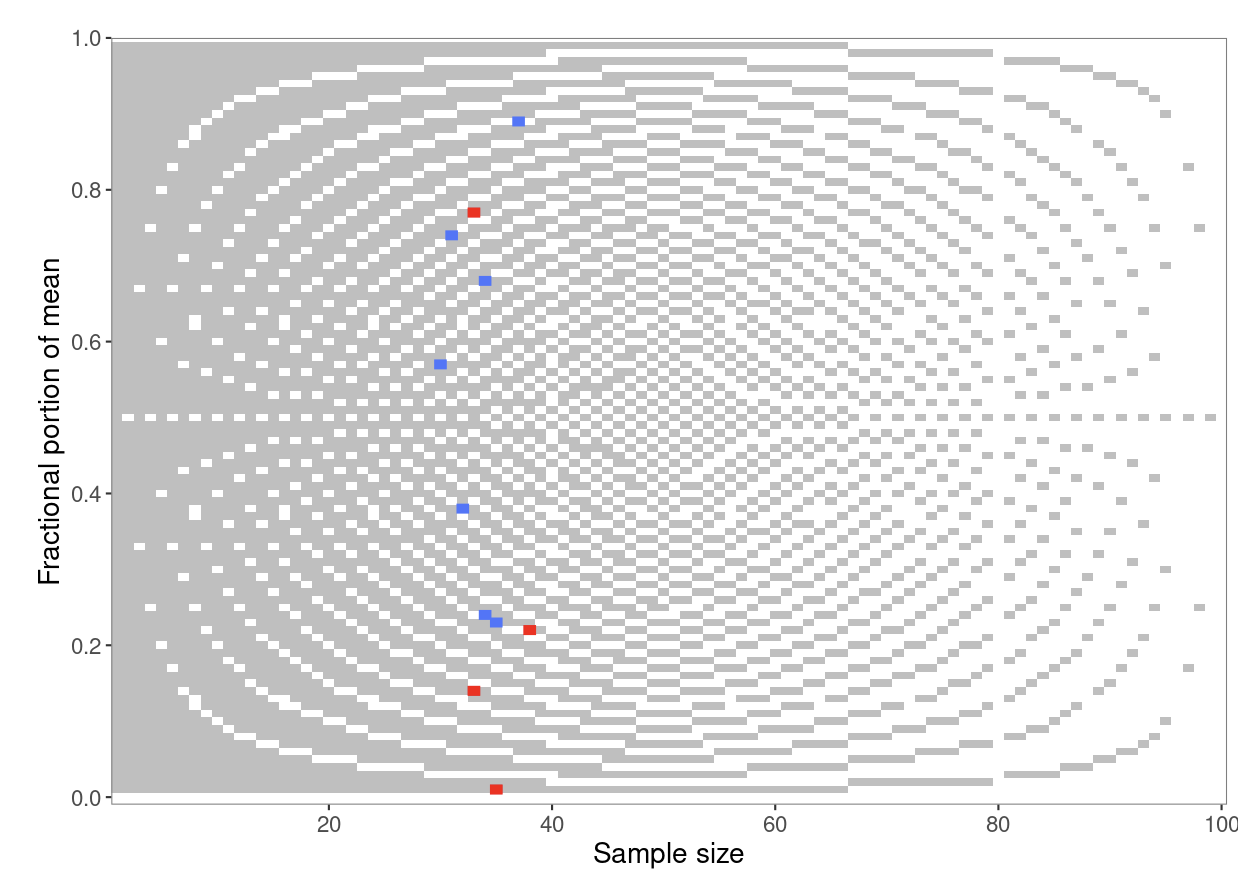
\includegraphics[width=0.5\linewidth]{img//granularity_testing_grim_grimmer/grim plot.png}
    \caption{Means that pass or do not pass GRIM based on sample size}
    \label{grimfig:figure-1}
\end{figure}
This insight is useful and important when interpreting the result of one or more GRIM test, especially when interpreting multiple values. It is important to consider not merely the proportion of values in an article that pass GRIM, but the difference between the baseline probability of passing GRIM at that sample size. For example, imagine that you extract 10 means from an article, all of which are based on a sample size of N = 70, and all of which are reported to two decimal places and were obtained using a single-item measurement instrument. If 7 out of 10 items pass GRIM, what should you infer about the means? The majority of the values passed GRIM, so a user may interpret this as evidence of the means' legitimacy. However, for this sample size and precision and granularity, 70\% of randomly generated means would pass GRIM. As such, the observed results are precisely in line with what would be observed with a set of generated by something other than a legitimate data generating process as described in the article, and would therefore be sufficient to mark the means as implausible within the context of a trustworthiness assessment. Additional information should then be sought from the authors regarding whether some unreported feature of the method could explain this pattern of results, as well as the raw data for further inspection. 

\subsection*{False negatives due to completely fabricated data}

It is important to recognize that GRIM/MER only tells you whether a reported mean (or other summary stat) could have been calculated from a given vector of observations. It tells you nothing about the provenance or legitimacy of the underlying data. In the extreme case of fabrication of an entire data set, the mean of those fabricated values can trivially pass GRIM. So, passing GRIM does not tell that the data is not fabricated, and failing it does not tell you it is fabricated. It merely tells you that description of the data generating process cannot produce the summary statistics that were reported. There are many reasons why these tests might fail, ranging from mere typos or the use of the wrong sample size (e.g., before vs. after exclusions) to fabrication of the reported results without any underlying dataset. 

\section*{Implementations}

There are multiple implementations of GRIM and GRIMMER available, with varying trade-offs between simplicity of use and complexity/reproducibility. 

\subsection*{nickbrown.fr/GRIM}

The simplest is probably \href{http://nickbrown.fr/GRIM}{Nick Brown's web app}, which has the benefit of being extremely simple, but does not contain documentation of how to use the tool or allow you to save its output in a reproducible way. Nick says he developed the web app to be able to run GRIM tests in real time when watching presentations at conferences.  

\begin{figure}[h!]
    \centering
    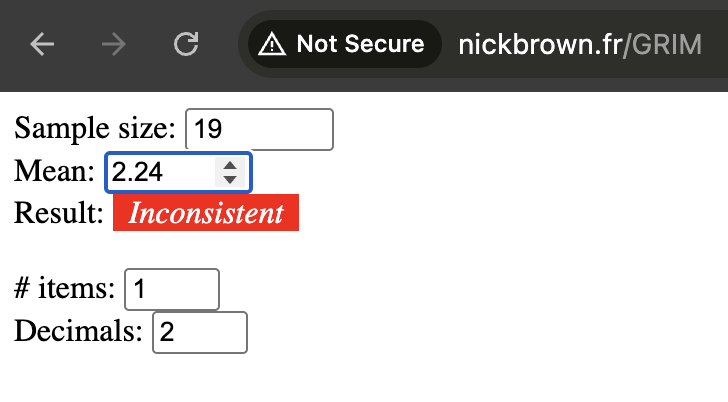
\includegraphics[width=0.5\linewidth]{nickbrown's grim test.png}
    \caption{Screenshot of Nick Brown's web app}
\end{figure}

\subsection*{{scrutiny} web app}

Lukas Jung's R package {scrutiny} also has an \href{https://errors.shinyapps.io/scrutiny}{R Shiny web app} that allows you to run GRIM and GRIMMER with a point-and-click graphical interface. This app has the benefit of allowing you to download a reproducible report of the results.

\begin{figure}[h!]
    \centering
    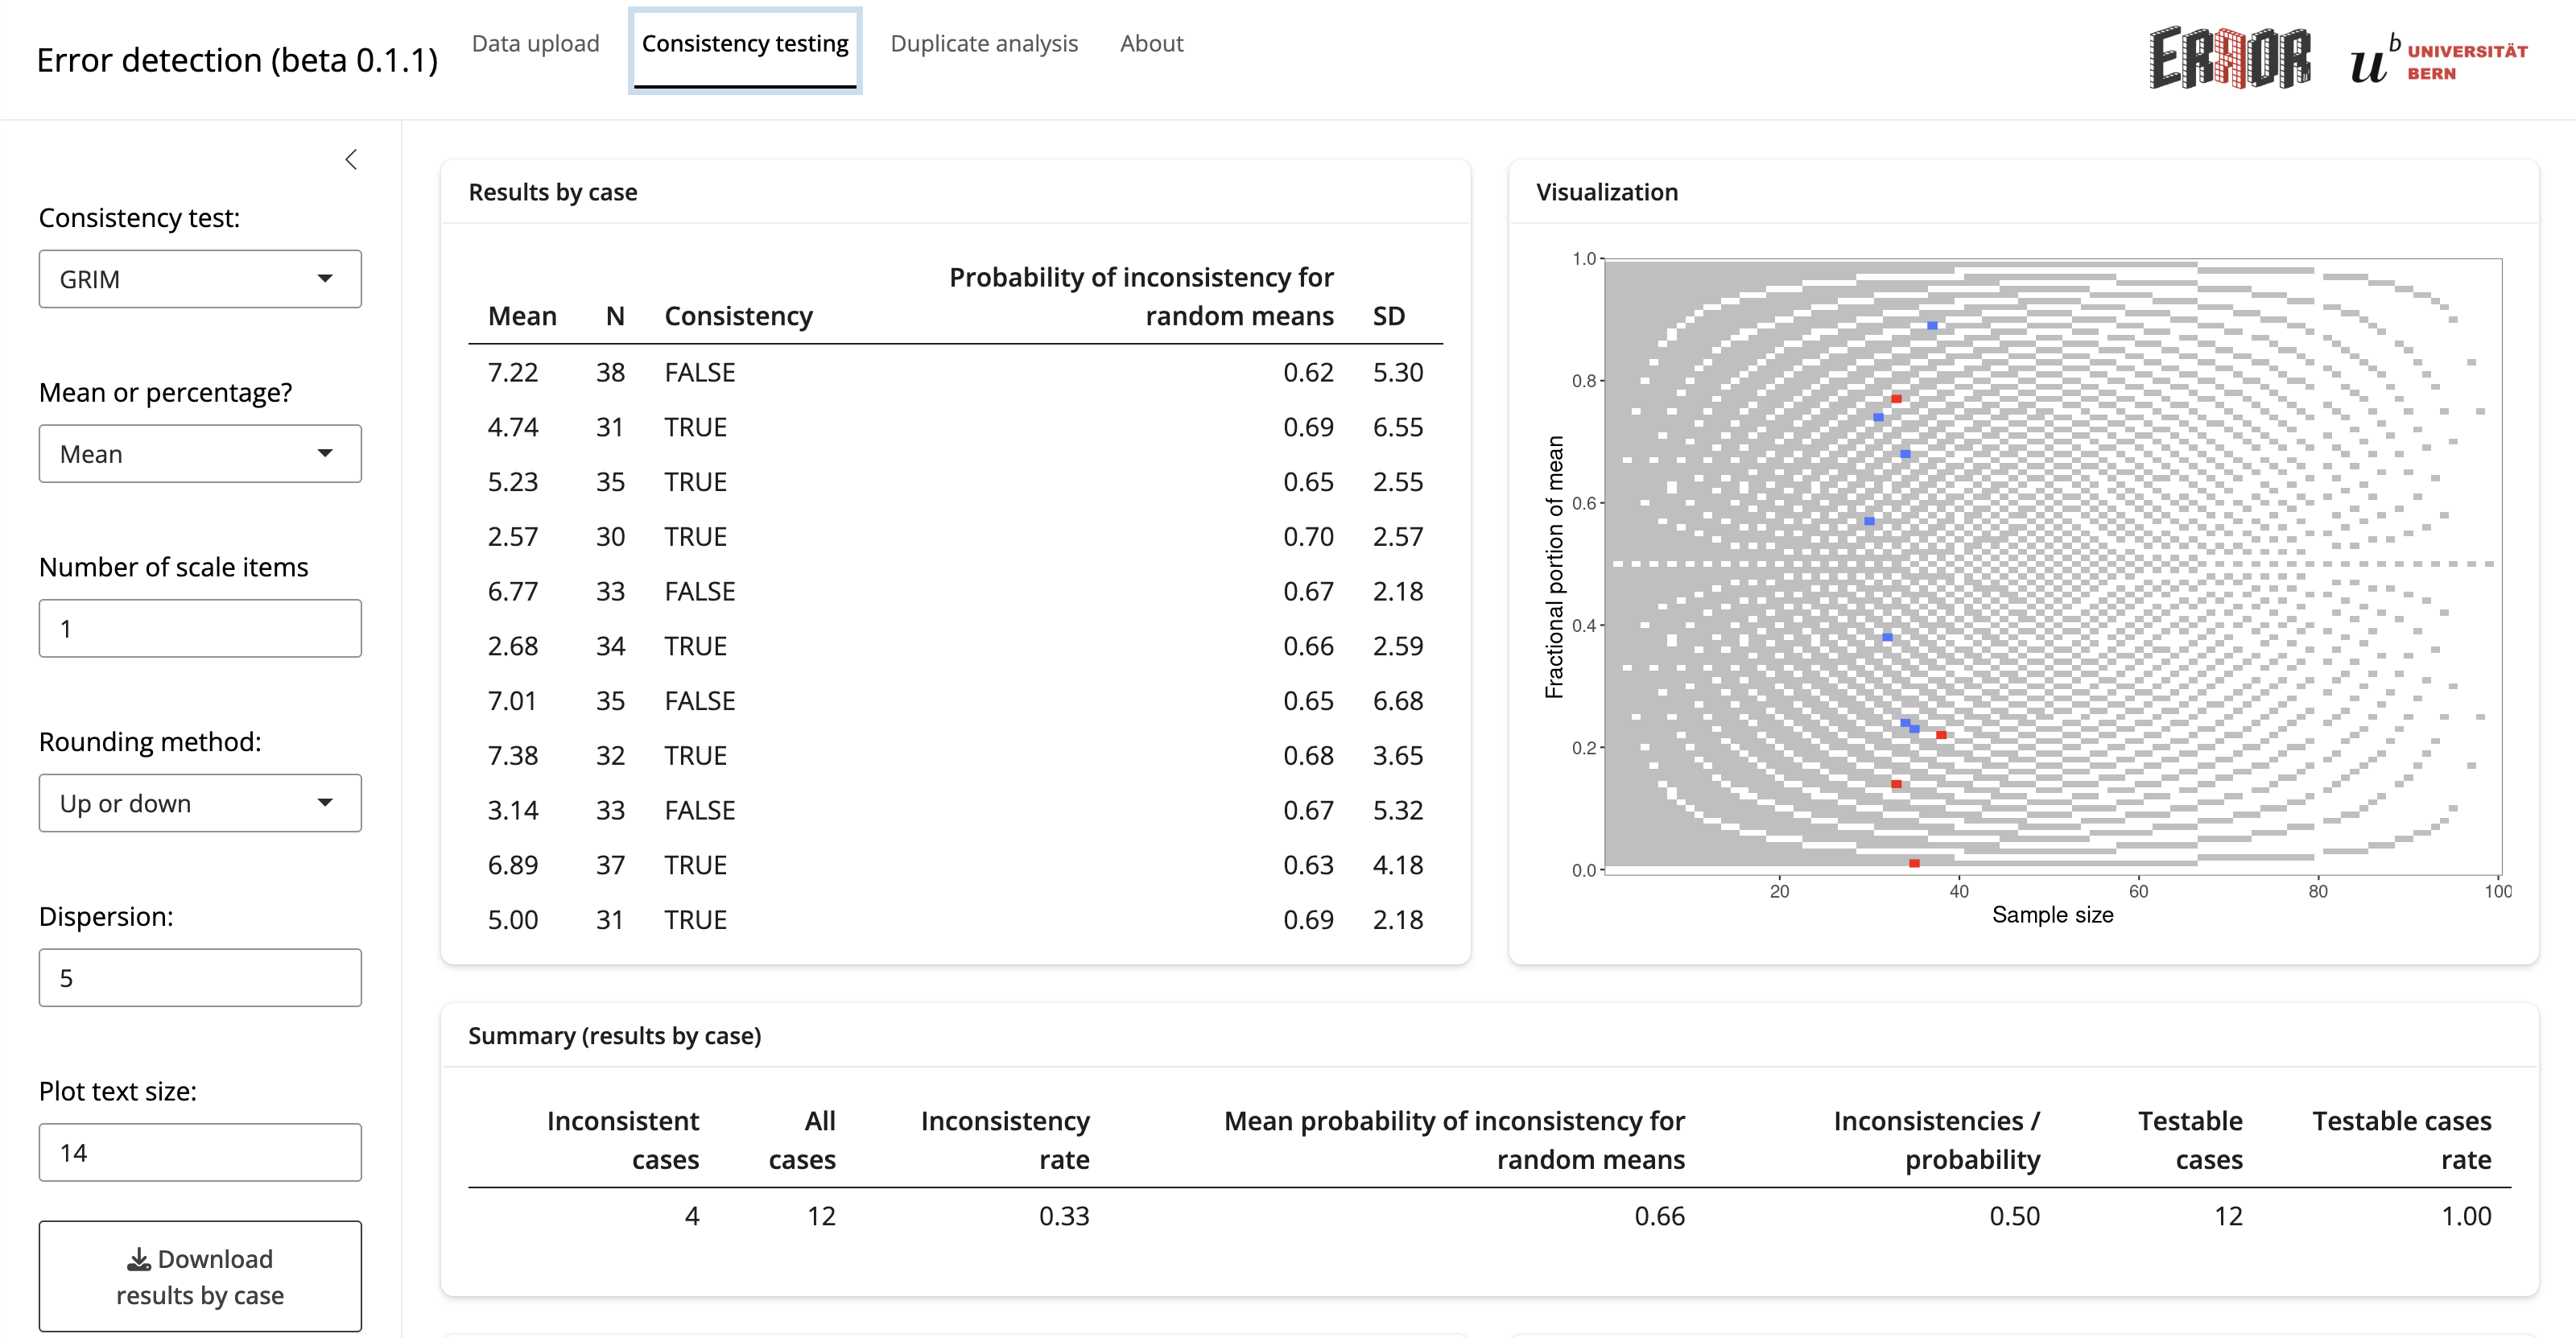
\includegraphics[width=0.5\linewidth]{scrutiny web app.png}
    \caption{Screenshot of Lukas Jung's web app}
\end{figure}

\subsection*{{scrutiny} R package}

Lukas Jung's R package {scrutiny} has an excellent implementation of GRIM and GRIMMER. See the \href{https://cran.r-project.org/web/packages/scrutiny/vignettes/grim.html}{vignette here}. GRIM can be run in one line of code as follows: 
\begin{verbatim}
library(scrutiny)
grim(x = "3.51", n = 30, items = 1)
\end{verbatim}
Using this R package has the benefit of allowing you to produce reproducible reports of results.

\subsection*{{rsprite2} R package}

Lukas Wallrich's {rsprite2} R package also contains an implementation of GRIM and GRIMMER. See \href{https://lukaswallrich.github.io/rsprite2}{package home page here}. GRIM can be run in one line of code as follows: 
\begin{verbatim}
library(rsprite2)
GRIM_test(mean = 3.51, n_obs = 30, n_items = 1)
\end{verbatim}
Using this R package has the benefit of allowing you to produce reproducible reports of results.

Note that during the last update of this guide, there are some values of SD that are GRIMMER consistent that \texttt{rscrutiny2::GRIMMER\_test()}currently returns as inconsistent. Therefore, it is recommended to use scrutiny over rsprite2 for GRIM/MER.

\subsection*{{grim} Python package}

Peter Houghton has also written an implementation of GRIM in Python, see \href{https://github.com/phoughton/grim_test}{here} or \href{https://pypi.org/project/grim/}{here}.
\begin{verbatim}
from grim import mean_tester
import decimal
print(mean_tester.consistency_check("3.51", "30", decimal.ROUND_HALF_UP))
\end{verbatim}

\section*{Additional Sources}
\begin{comment}
    

Allard, A. (2018) Analytic-GRIMMER: a new way of testing the possibility of standard deviations. https://aurelienallard.netlify.app/post/anaytic-grimmer-possibility-standard-deviations/

Anaya, J. (2016) The GRIMMER Test: A Method for Testing the Validity of Reported Measures of Variability. https://peerj.com/preprints/2400/

Brown, N., \& Heathers, J. (2017) The GRIM Test: A Simple Technique Detects Numerous Anomalies in the Reporting of Results in Psychology. \textit{Social Psychological and Personality Science.} https://doi.org/10.1177/1948550616673876

Heathers, J. (2016a) The GRIM test: a method for evaluating published research. https://jamesheathers.medium.com/the-grim-test-a-method-for-evaluating-published-research-9a4e5f05e870

Heathers, J. (2016b) The GRIM test: further points, follow-ups, and future directions. https://jamesheathers.medium.com/the-grim-test-further-points-follow-ups-and-future-directions-afd55ff67bb0#.vmgjvdvkf

Heathers, J. (2024) Using GRIM on intermediate figures to retrieve lost descriptive statistics. https://osf.io/m7j2r

Heathers, J. (2025a) An introduction to forensic meta-science. https://jamesheathers.curve.space

Heathers, J. (2025b) Approximately 1 in 7 scientific papers are Ffake. https://osf.io/5rf2m/
  - This article contains follow-up information related to Brown & Heathers (2017) related to potential cases of fraud that were uncovered by that earlier publication.

Hussey, I., Norwood, S. F., Cummins, J., Arslan, R. A., \& Elson, M. (2024). Truncation-Induced Dependency in Summary Statistics: A method for checking the compatibility of reported means, SDs, and Ns given the min and max of the scale. https://github.com/ianhussey/tides
  - Shiny web app: https://errors.shinyapps.io/TIDES/
\end{comment}

\begin{itemize}
    \item \href{https://aurelienallard.netlify.app/post/anaytic-grimmer-possibility-standard-deviations/}{Allard, A. (2018) Analytic-GRIMMER: a new way of testing the possibility of standard deviations.}

    \item \href{https://peerj.com/preprints/2400/}{Anaya, J. (2016) The GRIMMER Test: A Method for Testing the Validity of Reported Measures of Variability.}

    \item \href{https://doi.org/10.1177/1948550616673876}{Brown, N., \& Heathers, J. (2017) The GRIM Test: A Simple Technique Detects Numerous Anomalies in the Reporting of Results in Psychology. \textit{Social Psychological and Personality Science.}}

    \item \href{https://jamesheathers.medium.com/the-grim-test-a-method-for-evaluating-published-research-9a4e5f05e870}{Heathers, J. (2016a) The GRIM test: a method for evaluating published research.}

    \item \href{https://jamesheathers.medium.com/the-grim-test-further-points-follow-ups-and-future-directions-afd55ff67bb0#.vmgjvdvkf}{Heathers, J. (2016b) The GRIM test: further points, follow-ups, and future directions.}

    \item \href{https://osf.io/m7j2r}{Heathers, J. (2024) Using GRIM on intermediate figures to retrieve lost descriptive statistics.}

    \item \href{https://jamesheathers.curve.space}{Heathers, J. (2025a) An introduction to forensic meta-science.}
  
   \item \href{https://osf.io/5rf2m/}{Heathers, J. (2025b) Approximately 1 in 7 scientific papers are fake.}
% This article contains follow-up information related to Brown \& Heathers (2017) regarding potential cases of fraud that were uncovered by that earlier publication.

    \item \href{https://github.com/ianhussey/tides}{Hussey, I., Norwood, S. F., Cummins, J., Arslan, R. A., \& Elson, M. (2024) Truncation-Induced Dependency in Summary Statistics: A method for checking the compatibility of reported means, SDs, and Ns given the min and max of the scale.}

    \item \href{https://errors.shinyapps.io/TIDES/}{Shiny web app for TIDES.}
\end{itemize}
\end{document}